\chapter{Porte Logiche}

I circuiti digitali vengono realizzati utilizzando componenti chiamati \textbf{porte logiche}. Sono realizzate con componenti fisici come transistor e resistenze, ma nella progettazione dei circuiti digitali le porte logiche vengono schematizzate con i simboli riportati nella Figura 3.1 per semplificare la progettazione \textbf{astraendo} il livello di complessità della circuiteria analogica.
Solamente con la porta NAND si possono realizzare tutte le altre porte (NAND è funzionalmente completo), ma le porte in generale si costruiscono singolarmente con componenti appositi. Esse implementano la \textbf{logica booleana} che conseguentemente permette di realizzare operazioni di \textbf{aritmetica binaria} per costruire unità di calcolo in componenti elettronici e processori.

\begin{wrapfigure}{r}{0.6\textwidth}
	\begin{center}
		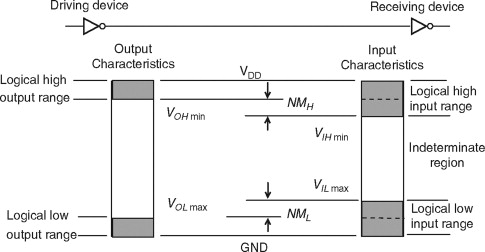
\includegraphics[width=0.58\textwidth]{noisemargin}
	\end{center}
	\caption{Margine di rumore nei circuiti digitali}	
\end{wrapfigure}


I componenti elettronici molto piccoli sono sensibili al \textbf{rumore}, per ovviare al problema i valori discreti (0 e 1) nei circuiti digitali non seguono un cambiamento istantaneo di differenza di potenziale (voltaggio), ma ammettono un margine per ridurre i problemi causati dal rumore.


I componenti (transistor) con cui si costruiscono porte logiche e circuiti sono realizzati con materiali semiconduttori, che possono essere di diversi tipi. Vedremo il tipo CMOS. Un transistor è composto da materiali come gallio e silicio.

\begin{wrapfigure}{r}{0.7\textwidth}
	\begin{center}
		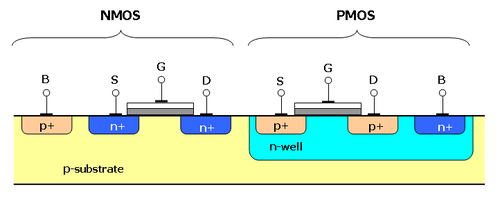
\includegraphics[width=0.68\textwidth]{cmos}
	\end{center}
	\caption{Transistor CMOS}
\end{wrapfigure}


\begin{figure}
	\centering
	\caption{Tabella delle porte logiche comuni}
	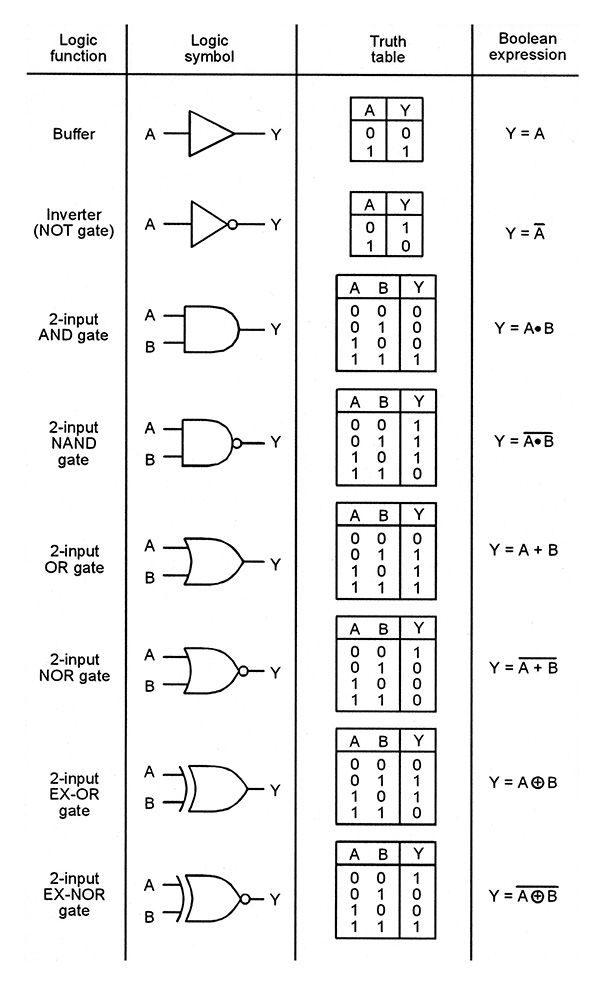
\includegraphics[width=\textwidth,height=\textheight]{logicgates}
\end{figure}
